% XeLaTeX. Editable vector plot; data embedded.
\documentclass[UTF8]{ctexart}
\usepackage[a4paper,landscape,margin=18mm]{geometry}
\usepackage{fontspec,pgfplots,caption}
\pgfplotsset{compat=1.18}\setmainfont{Times New Roman}\pagestyle{empty}
\definecolor{curveblue}{HTML}{287FA1}\definecolor{curveorange}{HTML}{EF8A32}
\begin{document}\begin{figure}[ht]\centering
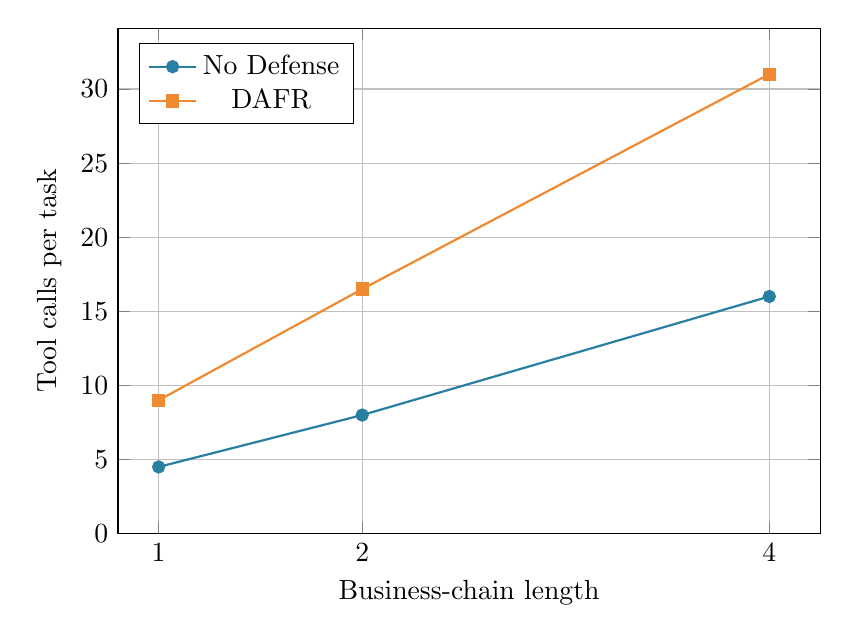
\begin{tikzpicture}\begin{axis}[width=10.5cm,height=8cm,xmin=.8,xmax=4.25,ymin=0,xtick={1,2,4},xlabel={Business-chain length},ylabel={Tool calls per task},grid=major,legend pos=north west]\addplot[thick,color=curveblue,mark=*] coordinates {(1,4.5) (2,8.0) (4,16.0)};\addlegendentry{No Defense}
\addplot[thick,color=curveorange,mark=square*] coordinates {(1,9.0) (2,16.5) (4,31.0)};\addlegendentry{DAFR}\end{axis}\end{tikzpicture}
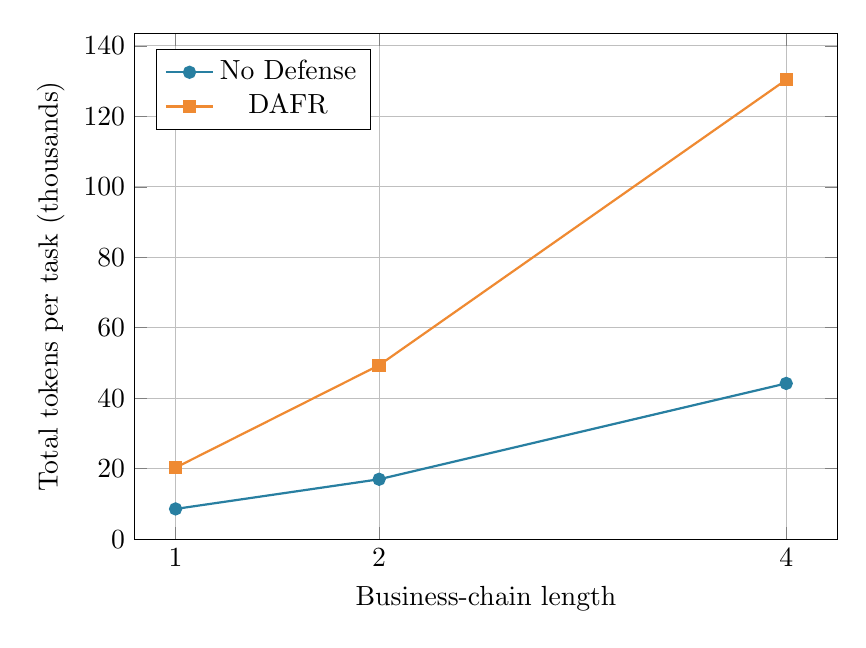
\begin{tikzpicture}\begin{axis}[width=10.5cm,height=8cm,xmin=.8,xmax=4.25,ymin=0,xtick={1,2,4},xlabel={Business-chain length},ylabel={Total tokens per task (thousands)},grid=major,legend pos=north west]\addplot[thick,color=curveblue,mark=*] coordinates {(1,8.587) (2,17.001) (4,44.2005)};\addlegendentry{No Defense}
\addplot[thick,color=curveorange,mark=square*] coordinates {(1,20.3015) (2,49.3685) (4,130.369)};\addlegendentry{DAFR}\end{axis}\end{tikzpicture}
\caption{同类任务不同业务链长的开销试验。科大 API 的 deepseek-v4-flash-ascend，在付款、文档授权两个实例上，分别执行 1、2、4 个依次解锁的业务操作；每个点为两个实例的平均值，总计 12 次执行。每条链仅在最后一个操作放置攻击，调用预算按链长同比增加。DAFR 平均工具调用数为 9、16.5、31，平均输入加输出 token 数为 20.3k、49.4k、130.4k。工具交互随链长近似线性增长，累计 token 增长更快。DAFR 六次均完成原任务并阻止攻击；No Defense 六次均任务失败且攻击成功。两条开销曲线对应不同质量的执行结果，不能据此视为等效任务完成的效率比较。}
\end{figure}\end{document}
